\documentclass[14pt,handout]{beamer}
%aspectratio=169
\usepackage[utf8]{inputenc}
\usepackage[T1]{fontenc}
\usepackage[magyar]{babel}
\usetheme{default}
\usepackage{subcaption} %subfigure

%\usepackage{pgfpages}
%\pgfpagesuselayout{4 on 1}[a4paper,border shrink=5mm]
% print with space for notes
%\usepackage{handoutWithNotes} 
% put 3 slides on 1 page with space for notes
%\pgfpagesuselayout{3 on 1 with notes}[a4paper, border shrink=5mm]

%oldalszam
\addtobeamertemplate{navigation symbols}{}{%
	\usebeamerfont{footline}%
	\usebeamercolor[fg]{footline}%
	\hspace{1em}%
	\insertframenumber/\inserttotalframenumber
}

%\usepackage{enumitem} %settings of itemize, e.g. itemsep


\title{Modell prediktív fűtésszabályozás alkalmazási lehetőségei}
\author{Gyulai László}
%\institute{Szakdolgozat bemutatás}
\date{2019. március 21.}

\newcommand\Fontvi{\fontsize{6}{7.2}\selectfont}


\usepackage{graphicx}
\usepackage{tikz}
\usetikzlibrary{mindmap,trees}
\usepackage{verbatim}

%\begin{document}
%	\pagestyle{empty}
	
	\begin{comment}
	:Title: Computer science mindmap
	:Tags: Manual, Mindmap
	
	Version 1.09 of PGF/TikZ added a library for drawing mindmaps. Here's an example
	from the manual. 
	
	| Author: Till Tantau
	| Source: The PGF/TikZ manual
	
	\end{comment}
	%\end{document}

\begin{document}
	
	\frame{\titlepage}
%\begin{frame}{Bevezető}
%
%%[shrink=-25]
%    \begin{itemize}
%        \item Témaválasztás szempontjai
%        \pause
%        \setlength{\itemsep}{6pt}
%        \begin{itemize}
%            \item szabályozástechnikai vonatkozás
%            \item gyakorlati haszon, piaci igény 
%        \end{itemize}
%    	\pause
%    	\item \underline{Korszerű fűtési rendszerek szabályozása}
%    	\pause
%        \begin{itemize}
%            \setlength{\itemsep}{3pt}
%        	\item a fenti kívánalmaknak megfelel
%        	        	
%	    	\item a témában érintett szakterületek:
%	    	\pause
%	        \begin{itemize}
%	            \item Épületgépészet
%	            \item Szabályozástechnika
%	            \item Jogszabályok, pénzügy és marketing 
%	            %környezetgazdaságtan
%	        \end{itemize}
%        \end{itemize}
%    \end{itemize}
%
%\end{frame}

\begin{frame}{A munka célja}
\begin{itemize}
	\setlength{\itemsep}{6pt}
	\item MPC szabályozás finomhangolása, továbbfejlesztése a szakdolgozat folytatásaként
	\item Költségek és a komfort közötti egyensúly	
	\item Különböző időállandójú beavatkozók használata
\end{itemize}
\end{frame}


\begin{frame}{MPC kutatások gyakorlati alkalmazással}
\begin{itemize}
	\setlength{\itemsep}{6pt}
	\item OptiControl projekt (Siemens, ETH Zürich, ...)
	\item \textbf{cél: }iroda integrált fűtés- és hűtésszabályozása
	\item \textbf{szenzorok: }hőmérsékletszenzorok, napsütés mérése, jelenlétérzékelés, stb...
	\item \textbf{szabályozás: } MPC, időjárás-jelentés adatokkal, többféle fűtési, hűtési módszerrel	

\end{itemize}
\end{frame}


\begin{frame}{Signal preview hatása MPC szabályozásra}
\begin{figure}[H]
	\centering
	% trim={<left> <lower> <right> <upper>}
	%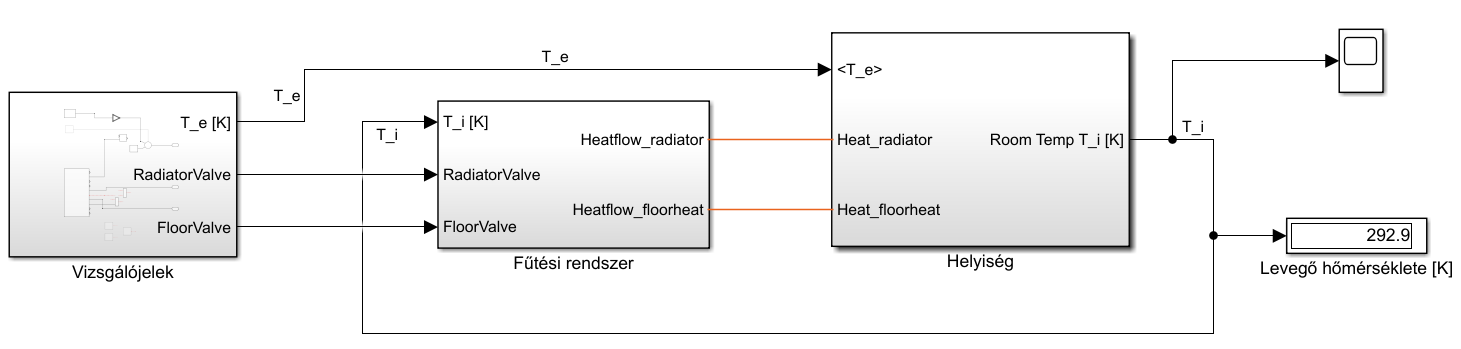
\includegraphics[trim=0 0 0 0, clip,width=\textwidth]{figures/simulink-network-minimalist-layout2}
	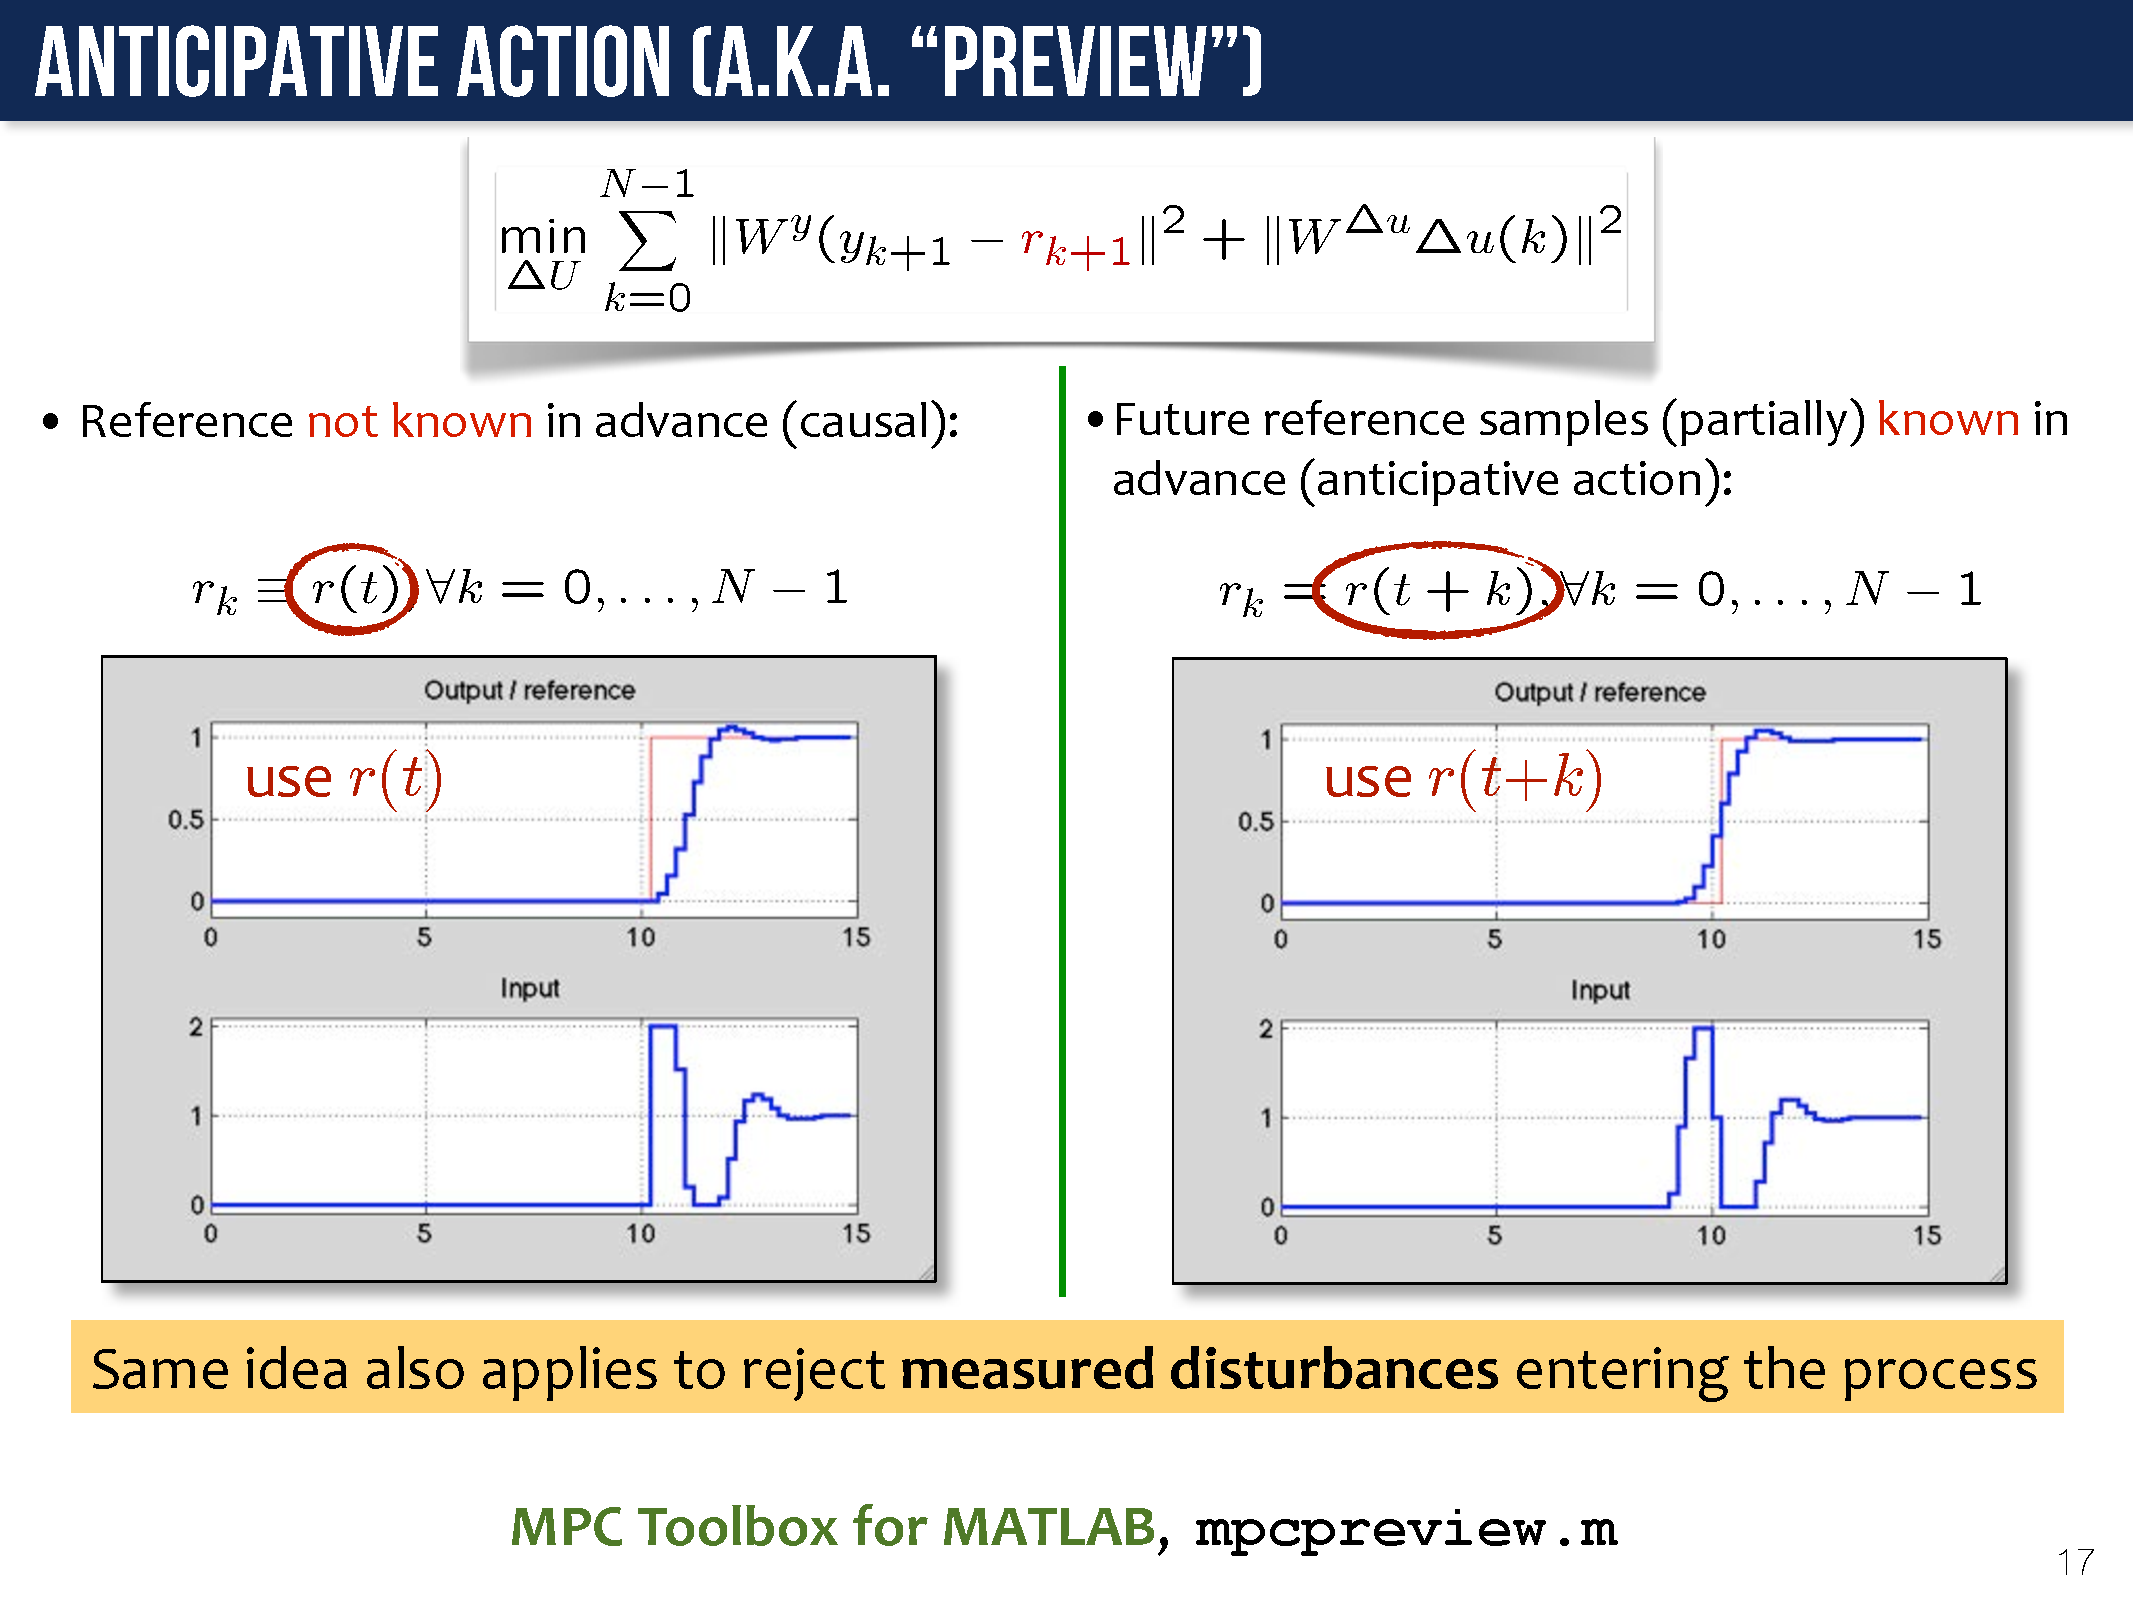
\includegraphics[trim=10 50 10 0, clip,width=\textwidth]{figures/onlab/preview}
\end{figure}
\end{frame}


\begin{frame}{Szimuláció}
\begin{figure}[H]
	\centering
	% trim={<left> <lower> <right> <upper>}
	%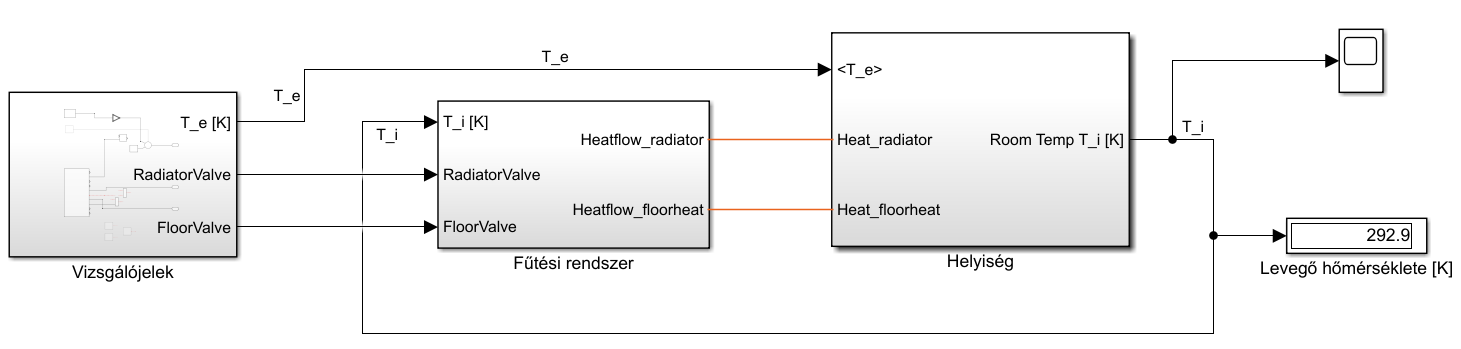
\includegraphics[trim=0 0 0 0, clip,width=\textwidth]{figures/simulink-network-minimalist-layout2}
	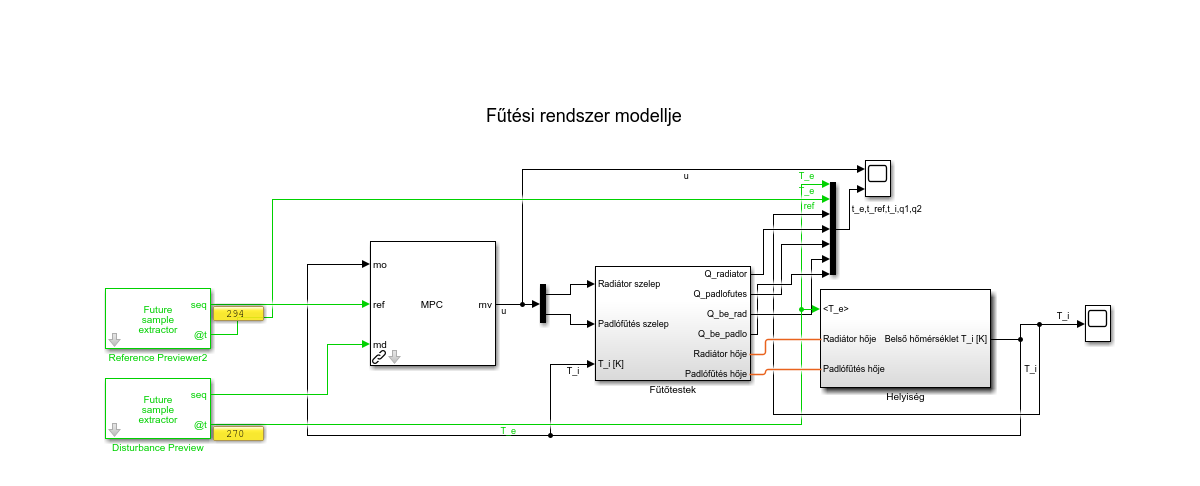
\includegraphics[trim=70 0 65 0, clip,width=\textwidth]{figures/onlab/comparepng}
\end{figure}
\end{frame}

\begin{frame}
\begin{figure}[H]
	\begin{subfigure}[t]{0.44\textwidth}
		\centering
		%	% trim={<left> <lower> <right> <upper>}
		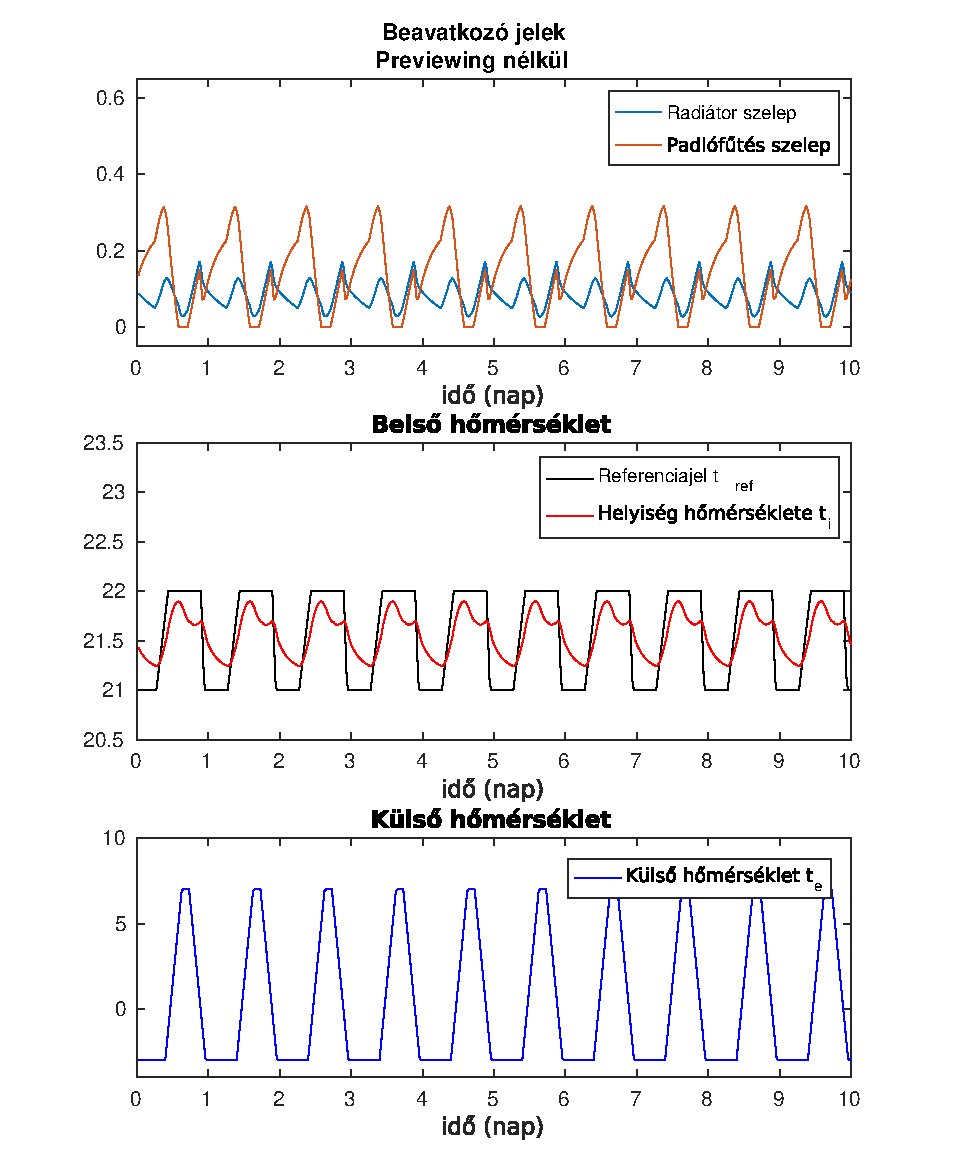
\includegraphics[trim=0 0 0 27, clip,width=\textwidth]{figures/onlab/compare/A_C_P0D0}
		\caption{\scriptsize Preview nélkül}
		\label{fig:mpc-pr0d0}
	\end{subfigure}
	~
	\begin{subfigure}[t]{0.47\textwidth}
		\centering
		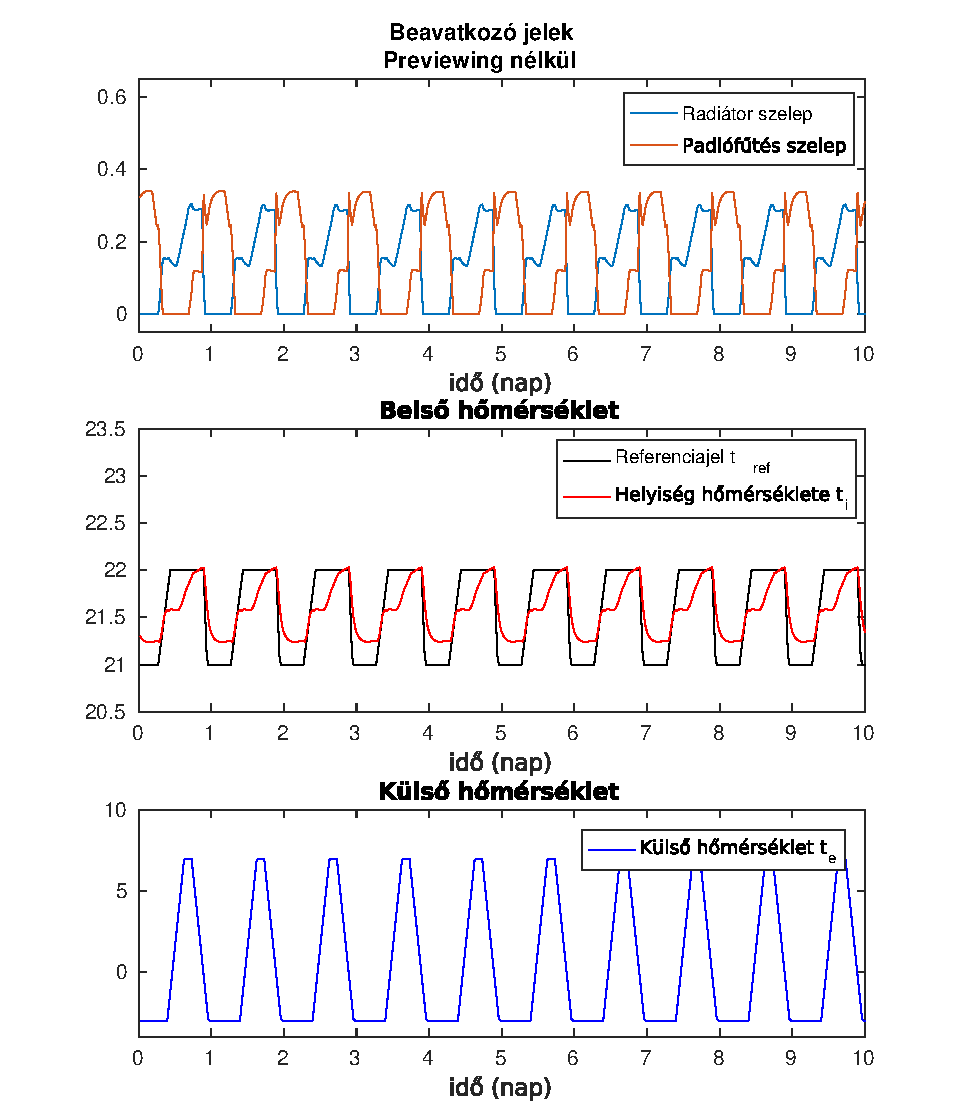
\includegraphics[trim=0 0 0 27, clip,width=\textwidth]{figures/onlab/compare/A_C_P0D10}
		\caption{\scriptsize Disturbance preview 10 step}
		\label{fig:mpc-pr0d10}
	\end{subfigure}
	\caption{MPC viselkedése -- previewing hatása}
	\label{fig:mpc-previeWeight}
\end{figure}
\end{frame}


\begin{frame}
\begin{figure}[H]
	\begin{subfigure}[t]{0.49\textwidth}
		\centering
		%	% trim={<left> <lower> <right> <upper>}
		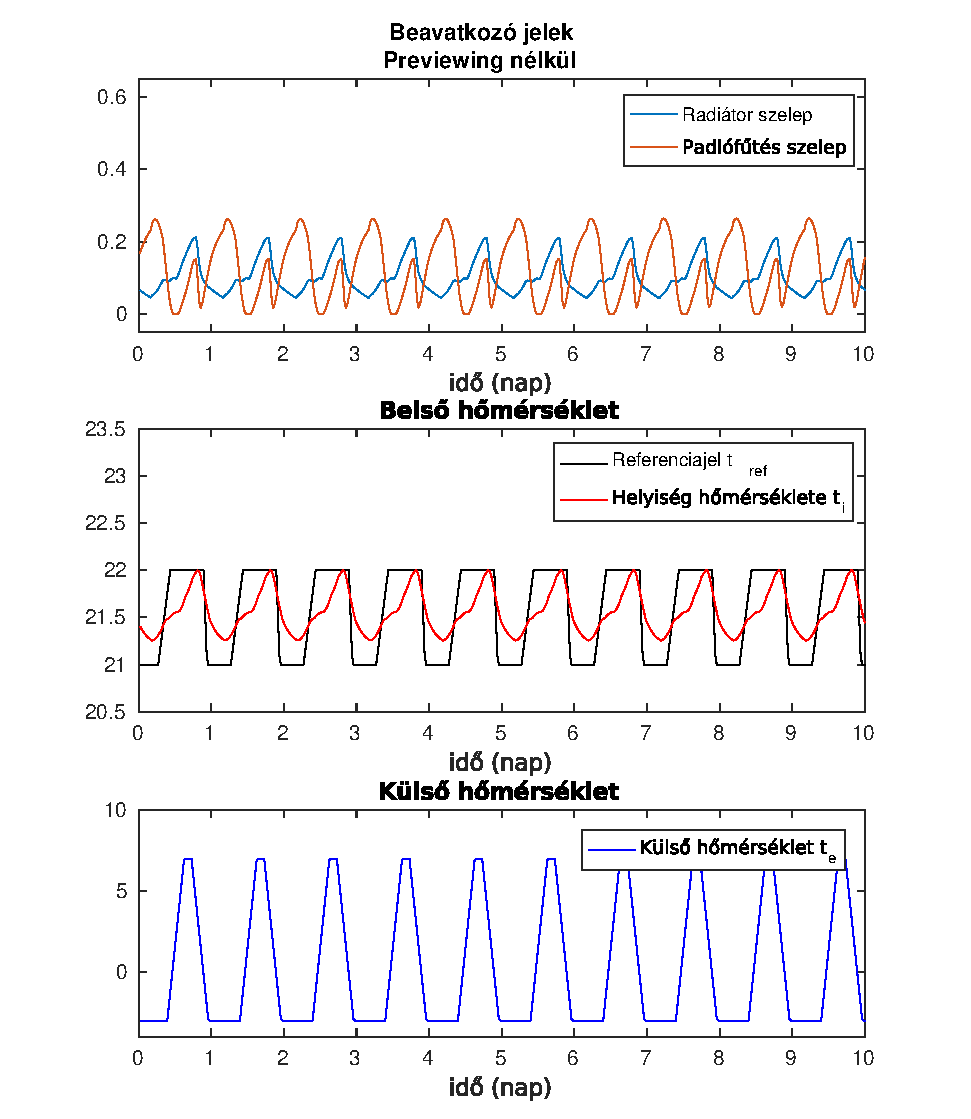
\includegraphics[trim=0 0 0 27, clip,width=\textwidth]{figures/onlab/compare/A_C_P5D10}
		\caption{\scriptsize Referencia 2.5 óra, zavarás 10 óra}
		\label{fig:mpc-pr5d10-2}
	\end{subfigure}
	~
	\begin{subfigure}[t]{0.45\textwidth}
		\centering
		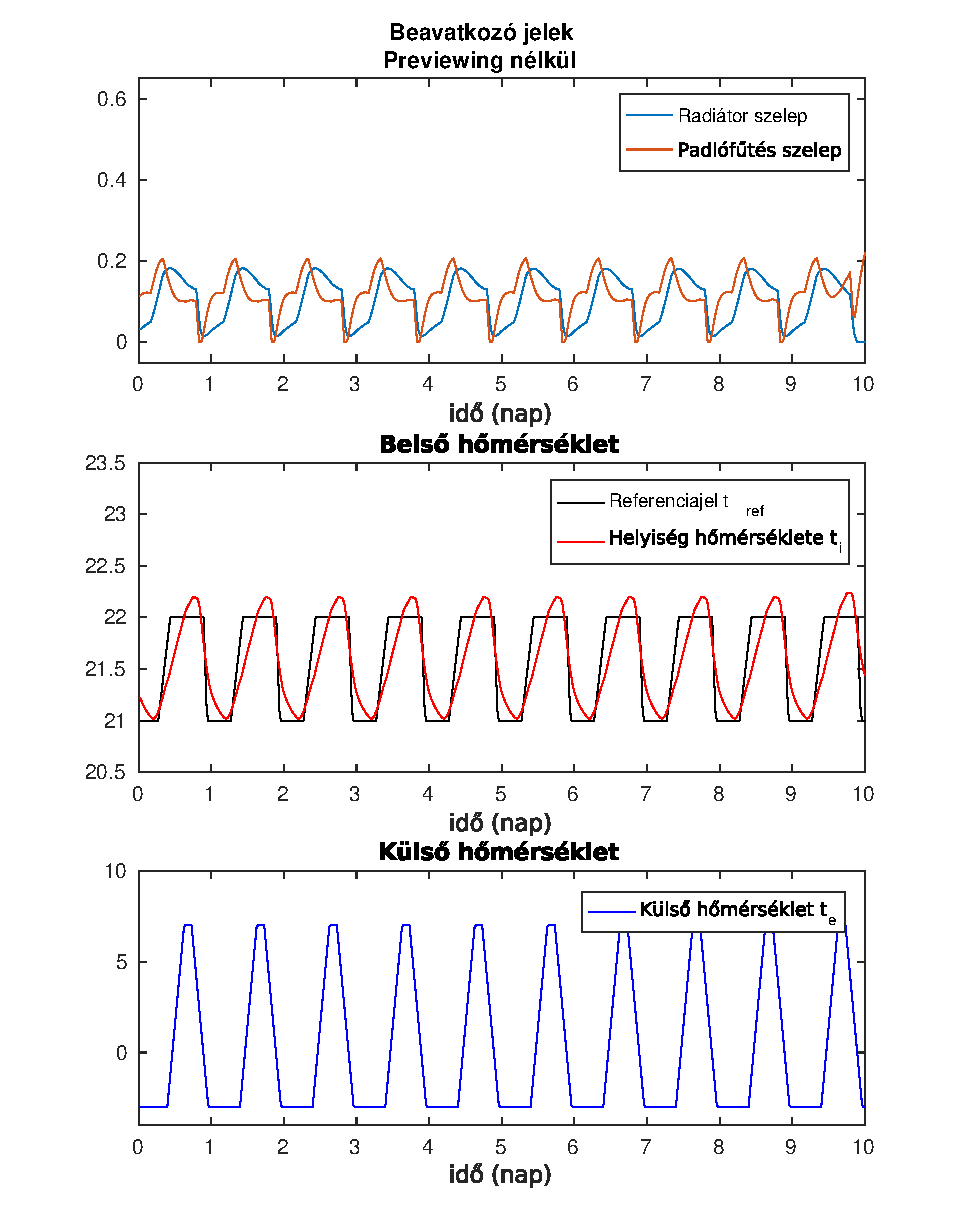
\includegraphics[trim=0 0 0 27, clip,width=\textwidth]{figures/onlab/compare/A_C_P5D48}
		\caption{\scriptsize Referencia 2.5 óra, zavarás 24 óra }
	\end{subfigure}
	\caption{MPC viselkedése -- previewing hatása}
	\label{fig:mpc-previeWeight2}
\end{figure}
\end{frame}

\begin{frame}
\begin{figure}[H]
	%	% trim={<left> <lower> <right> <upper>}
	\begin{subfigure}[t]{0.47\textwidth}
		\centering
		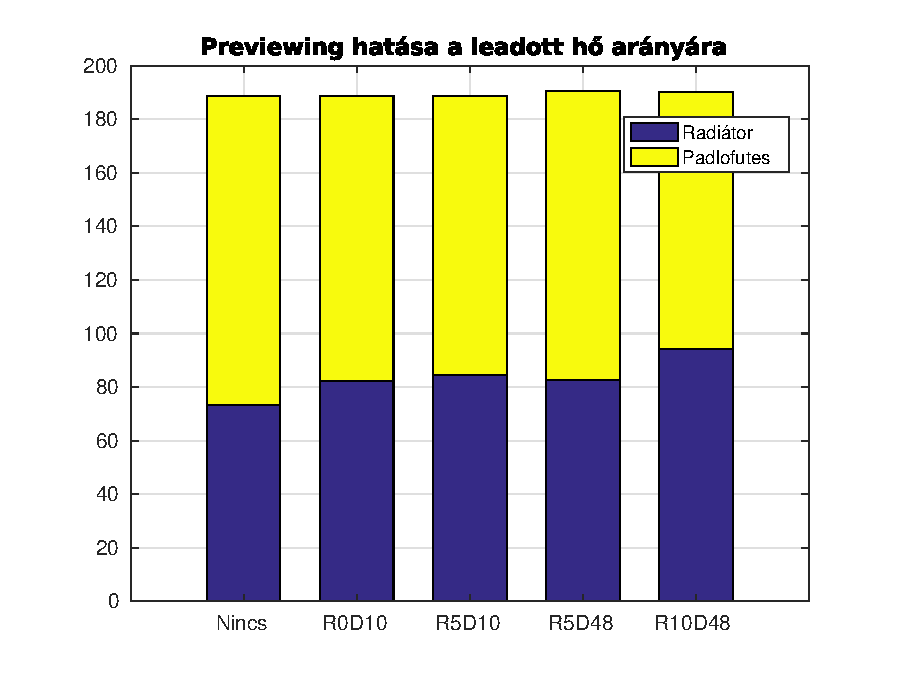
\includegraphics[trim=0 -40 0 0, clip,width=1.1\textwidth]{figures/onlab/compare/A_compareEnergy}
		\caption{Leadott hőmennyiség megoszlása a beavatkozók között}
		\label{fig:constrefHeat}
	\end{subfigure}
	~
	\begin{subfigure}[t]{0.47\textwidth}
		\centering
		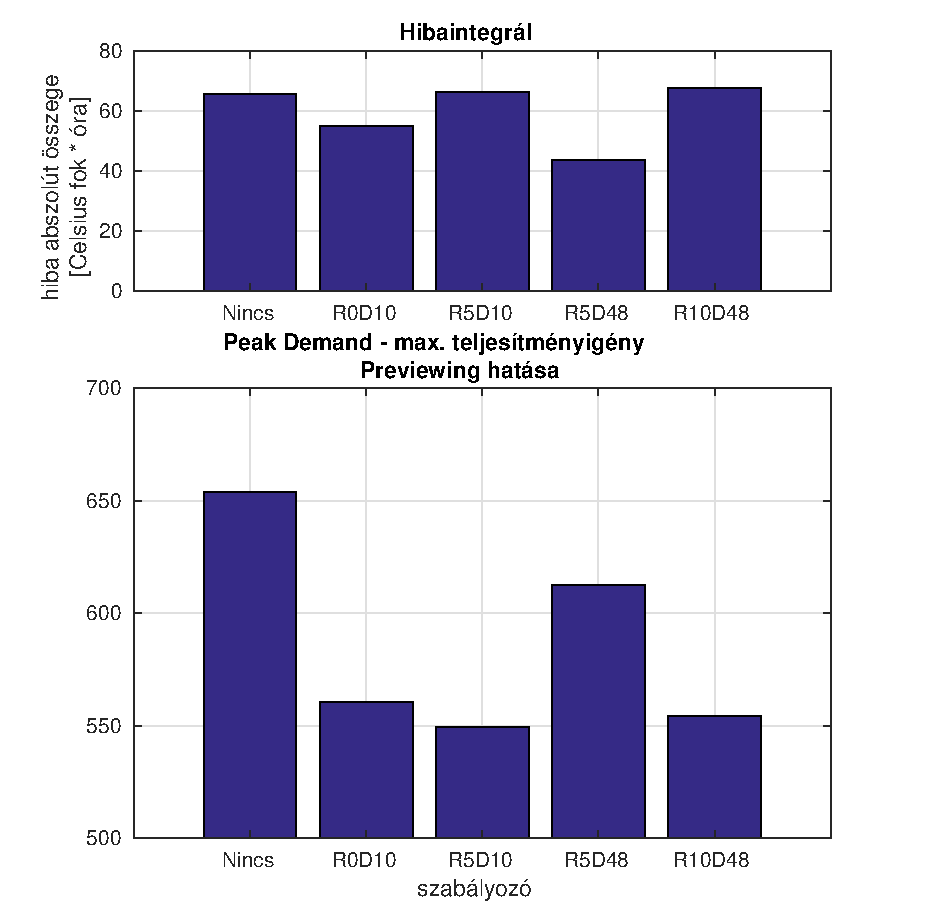
\includegraphics[trim=0 0 0 0, clip,width=1.1\textwidth]{figures/onlab/compare/A_compareComfort}
		\caption{Komfort (szabályozás hibája) és beavatkozójelek összege (max. teljesítmény)}
		\label{fig:mpc-PeakDemand}
	\end{subfigure}
	\label{fig:mpcComfortCost}
	\caption{Szabályozók összehasonlítása komfort és költség szempontjából}
\end{figure}
\end{frame}


\begin{frame}
\begin{figure}[H]
	\begin{subfigure}[t]{0.47\textwidth}
		\centering
		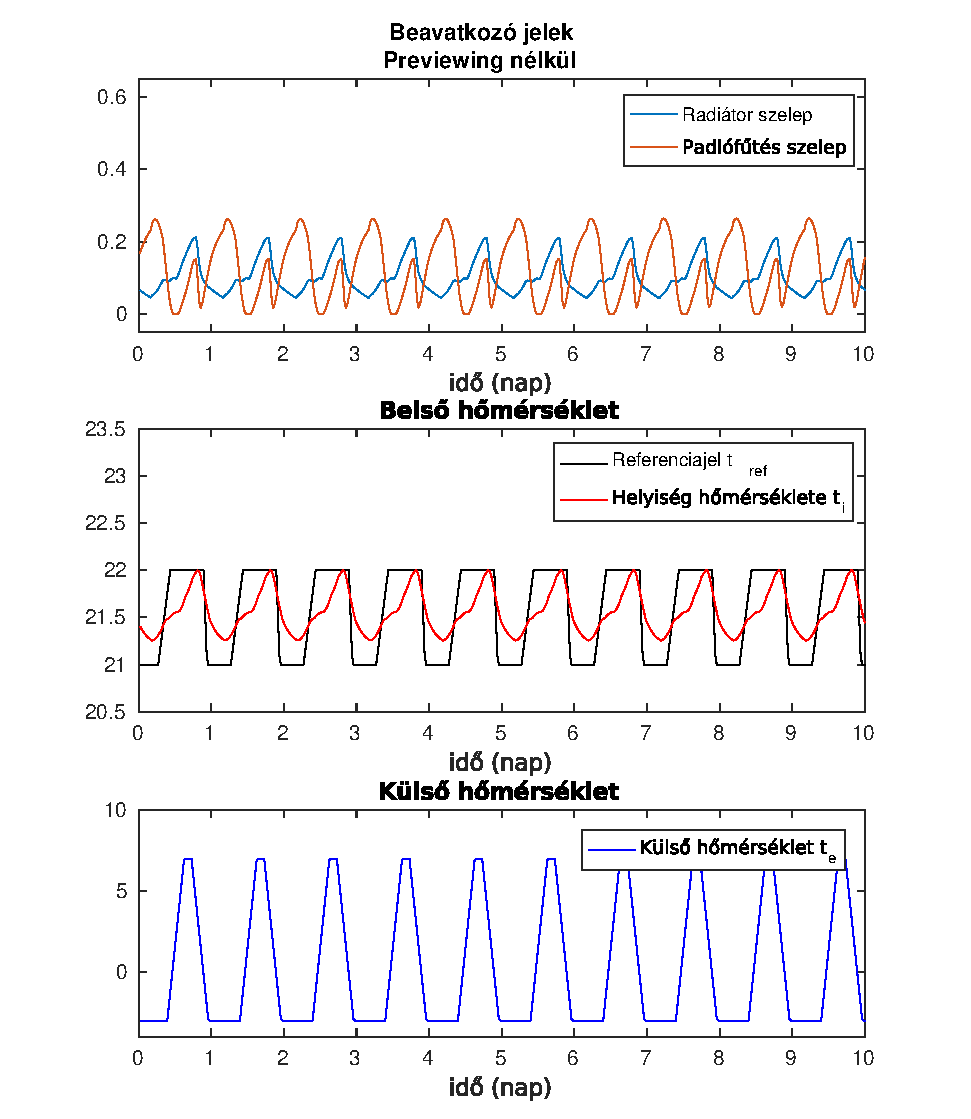
\includegraphics[trim=0 0 0 0, clip,width=\textwidth]{figures/onlab/compare/A_C_P5D10}
		\caption{Referencia 5 lépéssel, zavarás 10 lépéssel előre ismert}
		\label{fig:mpc-c-p5d10}
	\end{subfigure}
	~
	\begin{subfigure}[t]{0.47\textwidth}
		\centering
		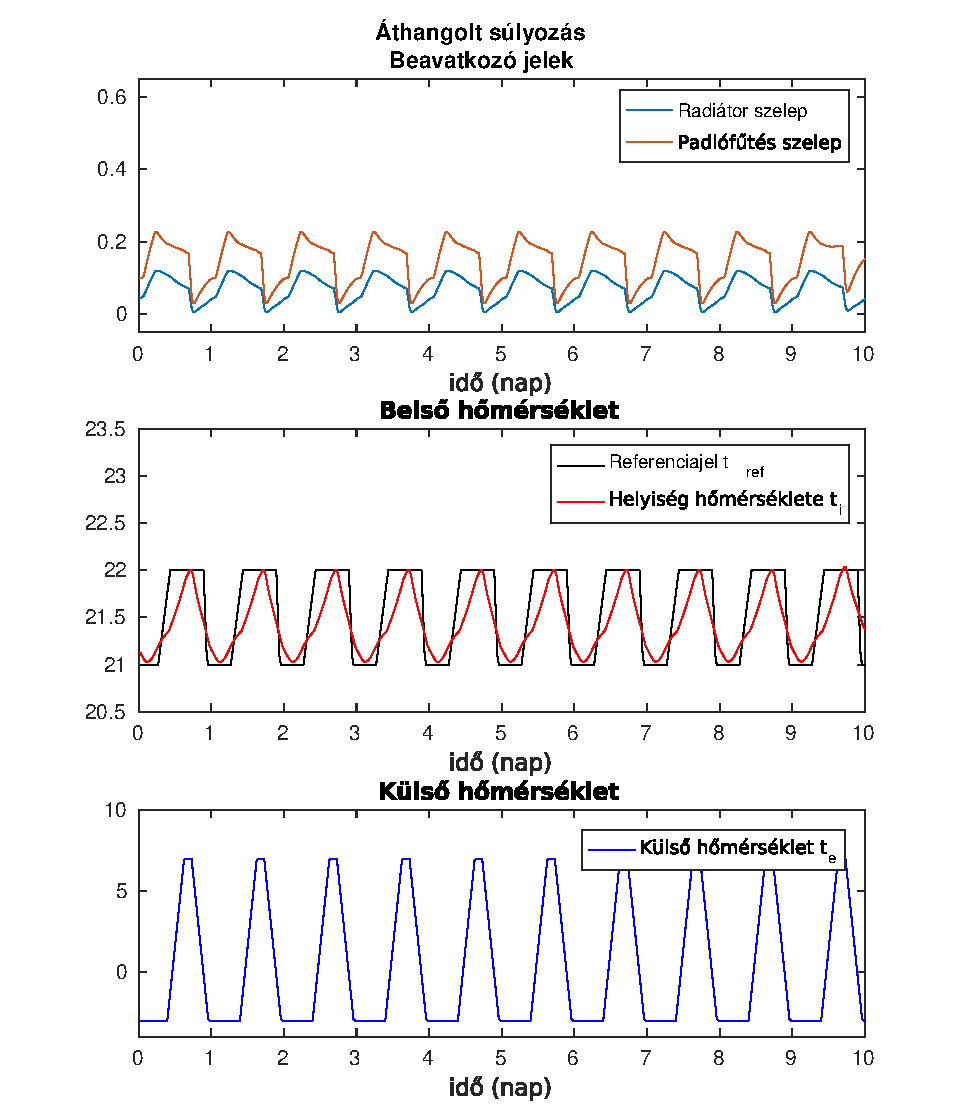
\includegraphics[trim=0 0 0 0, clip,width=\textwidth]{figures/onlab/compare/A_Cdiff_P10D48}
		\caption{Referencia 10 lépéssel, zavarás 48 lépéssel előre ismert, módosított súlyozással}
		\label{fig:mpc-cdiff-p10d48}
	\end{subfigure}
\end{figure}
\end{frame}


\begin{frame}
\begin{figure}[H]
	\begin{subfigure}[t]{0.47\textwidth}
		\centering
		%	% trim={<left> <lower> <right> <upper>}
		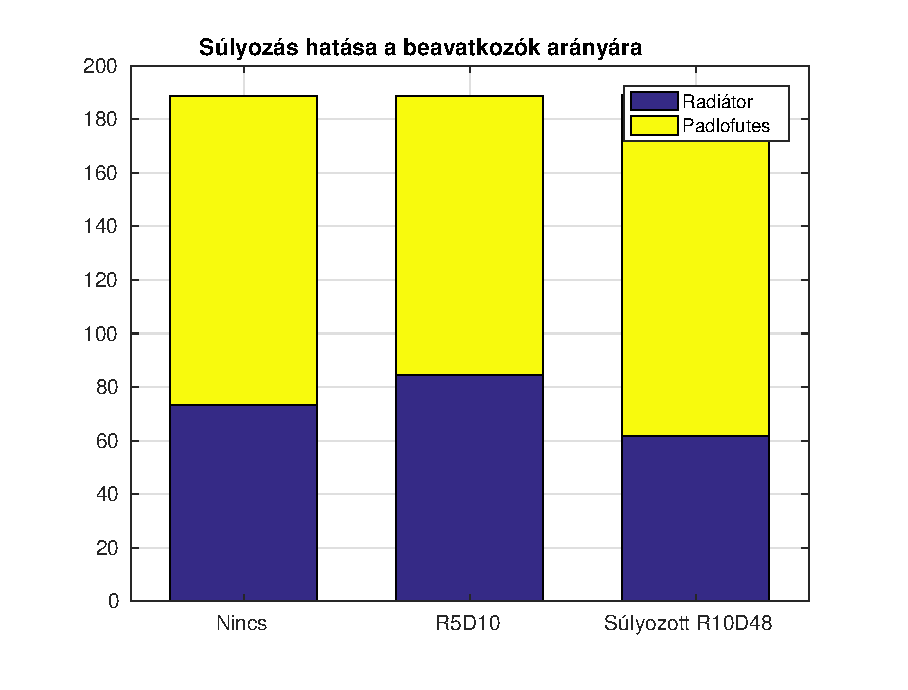
\includegraphics[trim=0 -40 0 0, clip,width=\textwidth]{figures/onlab/compare/A_diff_compareEnergy}
		\caption{Referencia 5 lépéssel, zavarás 10 lépéssel előre ismert}
		\label{fig:mpc-c-p5d10}
	\end{subfigure}
	~
	\begin{subfigure}[t]{0.47\textwidth}
		\centering
		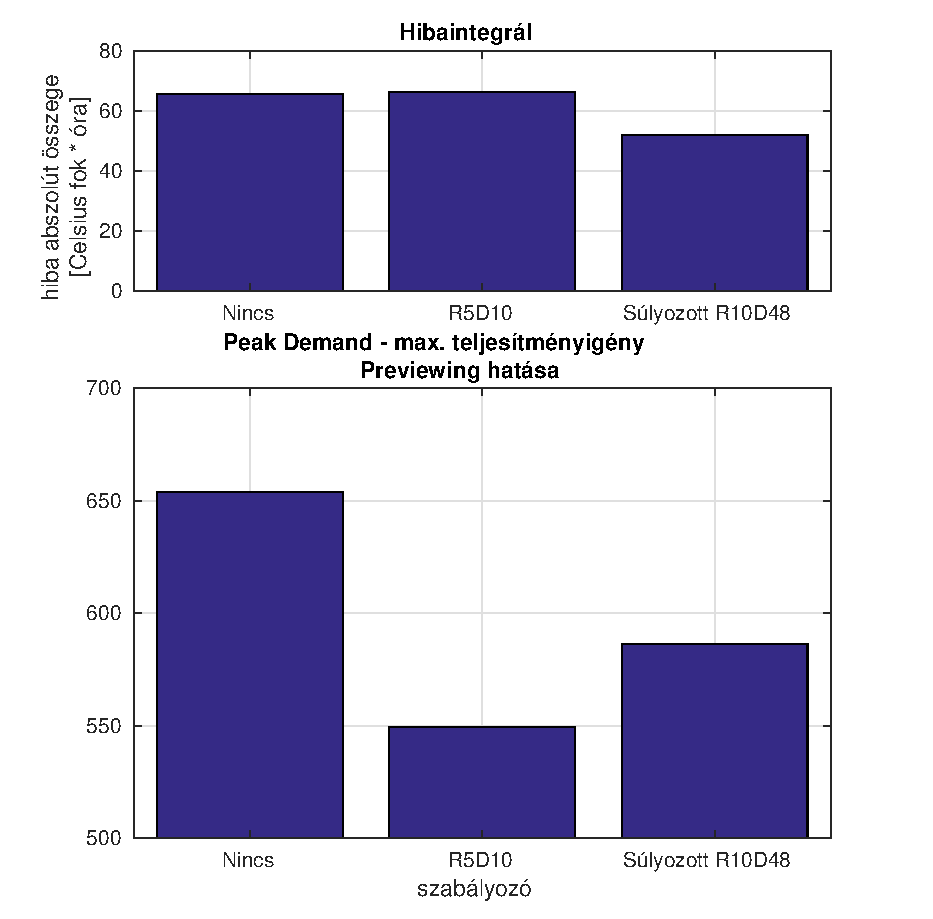
\includegraphics[trim=0 0 0 0, clip,width=\textwidth]{figures/onlab/compare/A_diff_compareComfort}
		\caption{Referencia 10 lépéssel, zavarás 48 lépéssel előre ismert, módosított súlyozással}
		\label{fig:mpc-cdiff-p10d48}
	\end{subfigure}
\caption{Súlyozás koorrigálása preview beállítása után}
\end{figure}

\end{frame}
%\begin{frame}{Műszaki tartalom}
%\Fontvi
%\centering
%\begin{tikzpicture}[thick,scale=0.7, every node/.style={scale=0.7}]
%\path[mindmap,concept color=black,text=white]
%node[concept] {\normalsize Termékfejlesztés}
%[clockwise from=-30]
%child[concept color=green!50!black] {
%	node[concept] {Tudás-\\vezérelt\\ötlet}
%	[clockwise from=0]
%	child { node[concept] {épületfizika} }
%	child {
%		node[concept] {szabályozástechnika}
%		[clockwise from=-45, level 3 concept/.append style={sibling angle=50, thick,scale=1.1}]
%		child { node[concept] {MIMO\\rendszerek} }
%		child { node[concept, scale=1.2] { \scalebox{0.9}{prediktív}\\ \scalebox{0.9}{szabályozás}} }
%	}
%	%child { node[concept] {pro\-gramming languages} }
%}  
%child[concept color=blue] {
%	node[concept] {applied}
%	%	[clockwise from=-30]
%	%	child { node[concept] {databases} }
%	%	child { node[concept] {WWW} }
%}
%child[concept color=red] {
%	node[concept] {Piacvezérelt\\ ötlet}
%	[clockwise from=-90]
%	child { node[concept] {törvényi \\ előírások} }
%	child { node[concept] {piaci \\ igények} }
%};
%\end{tikzpicture}
%\end{frame}
%
%
%
%


\begin{frame}{Eredmények értékelése}
\begin{itemize}
	\setlength{\itemsep}{6pt}
	\item A beavatkozók közti arány módosítható
	\item Csúcsidőben csökkenthető a teljesítményigény
	\item Megfelelő komfort -- költség egyensúly
\end{itemize}
\end{frame}


\begin{frame}{}
	\begin{center}
		\vspace{18pt}
		\large
		{\usebeamercolor[fg]{structure} 
			Köszönöm a figyelmet, \\
			várom a kérdéseket!
		}
	\end{center}
\end{frame}


\end{document}
